\documentclass[../main.tex]{subfiles}

\begin{document}
	
We have implemented a total of 5 methods for conducting inference as described in \autoref{sec:inference}.These models can be conceptually divided into  2 classes: bootstrap particle filtering based models (1,2) and rao-blackwellized particle filtering based models (3,4,5). In this section, we will compare and discuss the results obtained by the 5 inference algorithms. 

\begin{enumerate}
	\item A generic one-dimensional bootstrap particle filter (PF) which inferred only the returns ($x_2$) state.
	\item A drift-corrected bootstrap particle filter which infers both price ($x_1$) and returns ($x_2$) states simultaneously. 
	\item A Rao-Blackwellized Particle Filter (RBPF) for the case of a symmetrical \asd ($\beta = 0$)
	\item Dense Sampling improvement for the RBPF to reduce sample impoverishment 
	\item Adaptive Sampling improvement for the RBPF to create a fully adapted RBPF 
\end{enumerate} 

\textbf{Simulated Data Generation}

Unless explicitly stated, simulated data (with the simulation process described in \autoref{sec:experimental_simulated} has been used to obtain the results in this section. This provides us with both ground truth data for the states, as well as the actual parameters used, allowing us to test the effectiveness of the inference algorithms without the complications of parameter inference. The hyper-parameters used for generation of this simulated data is shown in Table \ref{tab:4__1__1__simulated_hyperparams}, and an example of the simulated data generated using these hyper-parameters is shown in Figure \ref{fig:4__1__1__simulated}.

\begin{table}[h!]
	\centering
	\begin{tabular}{lll}
		\toprule
		Parameter & Description & Value \\
		\midrule
		$\alpha$	& \asd tail exponent 		& 1.2 	\\
		$\beta$		& \asd skewness parameter 	& 0 	\\
		$\sigma$	& \asd volatility 			& $2 \times 10^{-4}$ \\
		$\sigma_{obs}$ & observation noise		& $2 \times 10^{-1}$ \\
		$\theta$	& mean reversion coefficient & -0.05 \\
		$\delta t$  & time gap between observations & 1 \\
		$T$			& Number of time steps		& 1500 \\
		\bottomrule
	\end{tabular}
	\caption{Hyper-parameters used for simulated data}
	\label{tab:4__1__1__simulated_hyperparams}
\end{table}

\begin{figure}[h!]
	\centering
	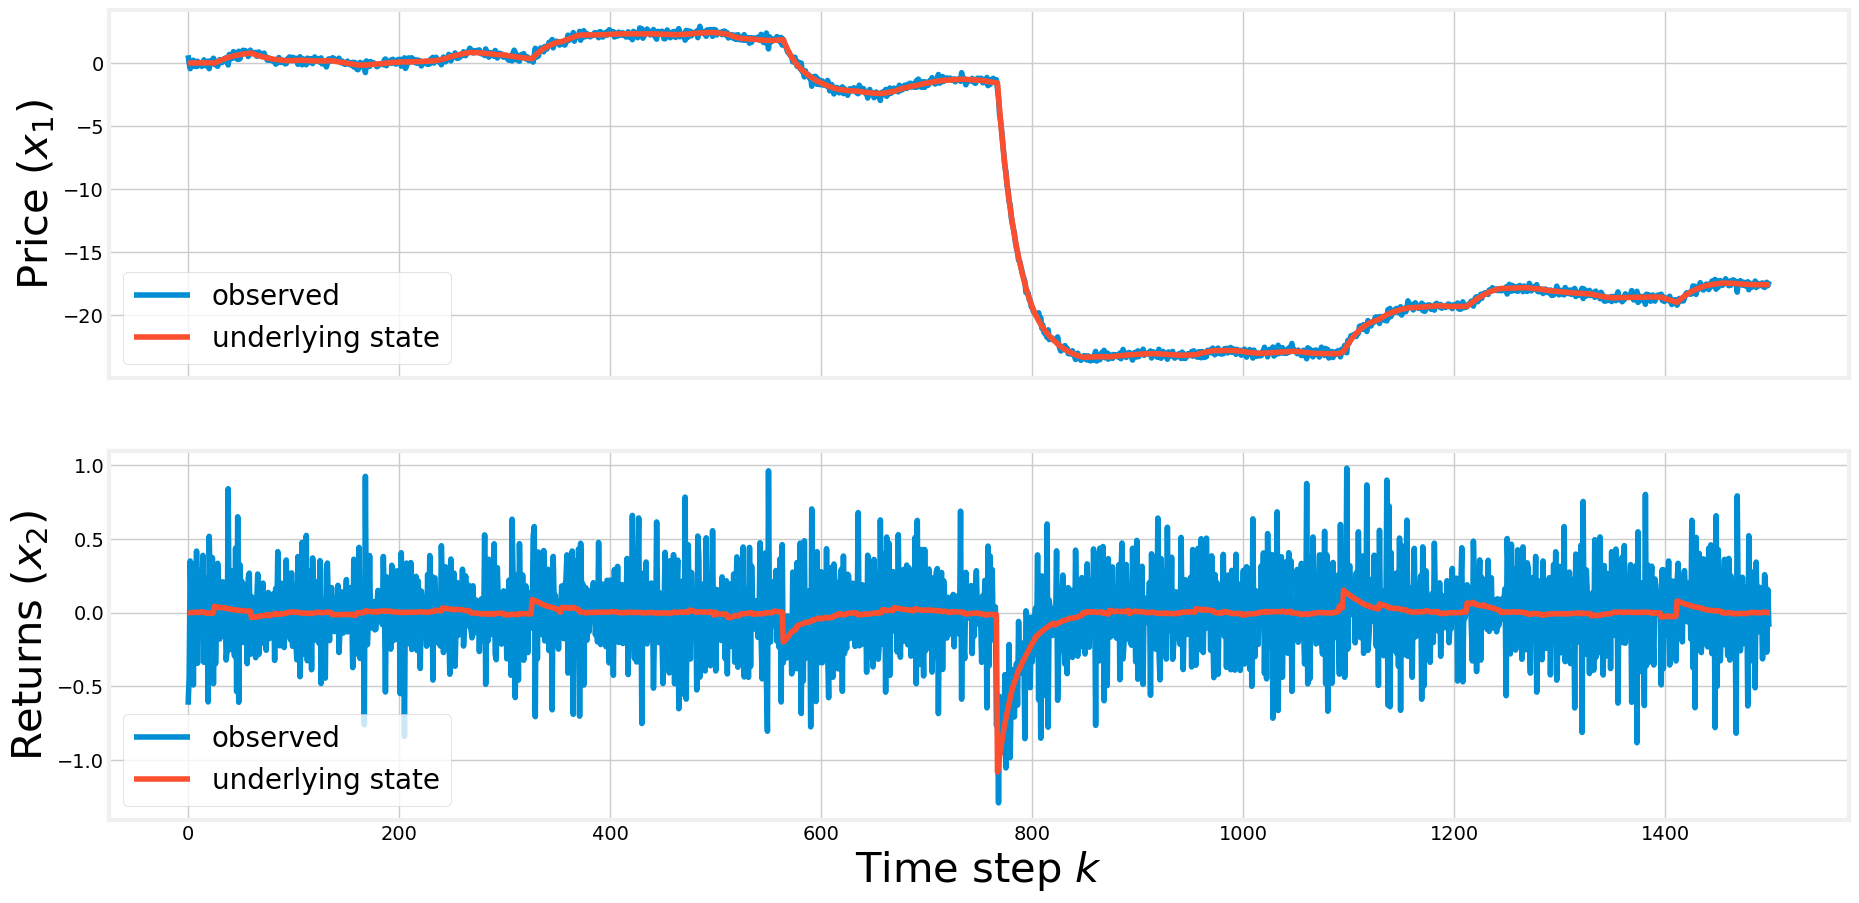
\includegraphics[width=15.0cm]{../plots/4__1__1__simulated.png}
	\caption{Example of simulated data}
	\label{fig:4__1__1__simulated}
\end{figure}

\textbf{Overall Comparison}

As a brief comparison of all the 5 inference algorithms, Figure \ref{fig:4__1__comparison} shows the performance of all 5 inference algorithms using a large number of particles ($N=10000$). We can observe that the RBPF based particle filtering based algorithms perform better in general than the bootstrap particle filtering based algorithms in terms of the Root Mean Square Error (RMSE) of both the underlying price and returns state. This continues to hold true even for lower number of particles. We will now compare the performance of the 2 classes of inference algorithms separately to allow for a more detailed comparison of the inference performance of each algorithm.

\begin{figure}[h!]
	\centering
	\subfloat[Root Mean Square Error (RMSE) of the price($x_1$) process \label{fig:4__1__comparison_price}]{
		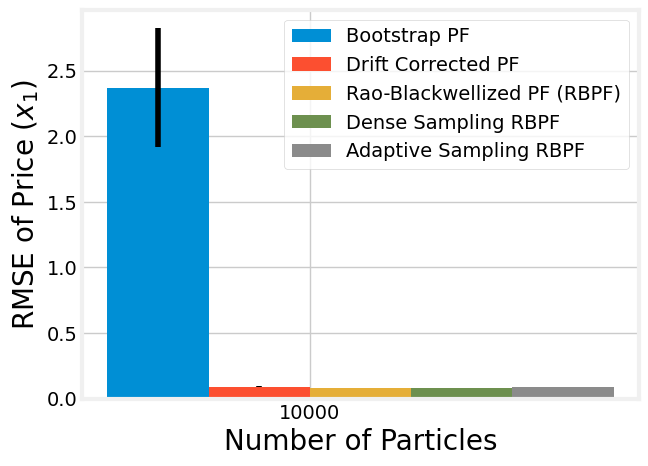
\includegraphics[height=4.5cm]{../plots/4__1__comparison_price.png}}
	\qquad
	\subfloat[Root Mean Square Error (RMSE) of the returns($x_2$) process  \label{fig:4__1__comparison_returns}]{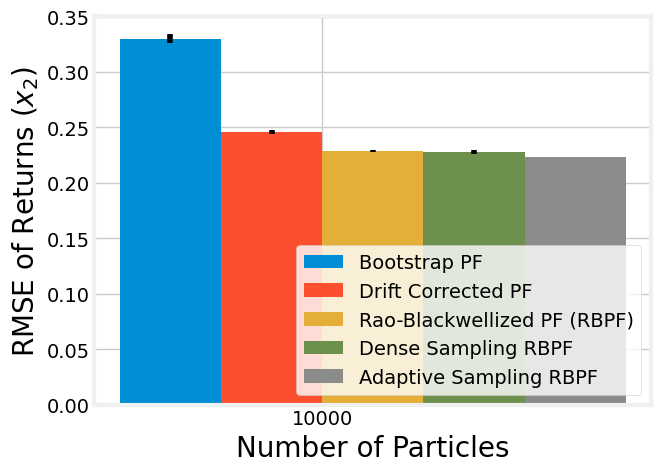
\includegraphics[height=4.5cm]{../plots/4__1__comparison_returns.png}}
	\caption{Comparison of all inference algorithms, $N = 10000$ particles}
	\label{fig:4__1__comparison}
\end{figure}

\textbf{Comparison of Bootstrap Particle Filters}

Firstly, we note that the generic one dimensional bootstrap particle filter performs very badly in tracking the underlying price state, as can be seen from Figure \ref{fig:4__1__1__bootstrap_comparison_rmse_price}. With a larger number of particles, the drift-corrected bootstrap particle filter is significantly better at tracking the underlying price state. 

However, both algorithms perform almost just as well at inferring the underlying returns state, although the RMSE of the drift-corrected particle filter when tracking the underlying returns state exhibits large variability for low number of particles. This is likely due to the drift-corrected particle filter being very sensitive to sample impoverishment in the same manner as described in \autoref{sec:inference_RBPF}. 

For low $N$ and large $\vt$, the samples of $\bvec{x}_k$ obtained from the particle filter proposal distribution are likely to have very low acceptance weights, resulting in a lack of particles with effective weights. If there are no particles with effective weights generated by the particle filter, the tracking performance of the particle filter can be severely diminished. The larger the observed price outlier ($\vt$) and the lower the number of particles $N$, the greater the impact of this problem and the less likely that particles with effective weights will be generated.

Due to sample impoverishment, we expect the performance of the bootstrap particle filters to fall rapidly as the number of particles drops. Furthermore, we also expect the RMSE achieved by the bootstrap particle filters to be more variable at low numbers of particles. This effect can be seen in Figure \ref{fig:4__1__1__bootstrap_comparison_rmse_price} and \ref{fig:4__1__1__bootstrap_comparison_rmse_returns}.

Lastly, we note that the Binary Prediction Error (BPE) of the returns process is much less affected by low numbers of particles as compared to the RMSE. Optimising for BPE only requires the particle filter to predict the correct \textit{direction} of returns, and is hence a less challenging task compared to accurately forecasting the underlying return state (measured by RMSE). This is encouraging, as it implies that the actual trading performance of the particle filters is likely to be less affected by random initialisations of the particles filter, and hence is likely to be more robust to outliers in the data. 

For $N=1000$ and $N=10000$, we also note that the BPE (0.25) is much lower than a BPE based solely on change (0.5), indicating that the bootstrap particle filters are frequently able to correctly predict the direction of the underlying return state. This is encouraging, and suggests that trading algorithms based on these filters will be profitable.

\textbf{Comparison of Rao-Blackwellized Particle Filters}

Figures \ref{fig:4__1__1__RBPF_comparison_rmse_price}, \ref{fig:4__1__1__RBPF_comparison_rmse_returns} and \ref{fig:4__1__1__RBPF_comparison_bpe_returns} show how the performance of the 2 bootstrap particles filters varies as the number of particles, $N$ is changed. 

Firstly, we note that the performance of the 3 RBPF-based particle filters is in general better than the bootstrap particle filters across all performance metrics. This suggests that the ability of the RBPF-based particle filters to marginalise out the gaussian components of the hidden state is very useful in improving the inference performance of the particle filter. 

Secondly, we note that in general, the performance of the dense sampling RBPF and the adaptive sampling RBPF are both slightly better than that of the generic RBPF, suggesting that the dense sampling and adaptive sampling improvements are both useful in improving the inference performance of the generic RBPF. Figures \ref{fig:4__1__1__RBPF_comparison_rmse_price} and \ref{fig:4__1__1__RBPF_comparison_rmse_returns} indicate that the performance of the generic RBPF degrades significantly as the number of particles ($N$) used drops, likely due to sample impoverishment. However, the dense sampling RBPF and adaptive sampling RBPF are both more resistant to this degradation in performance, indicating that they are likely less affected by sample impoverishment. 

In particular, the adaptive sampling RBPF is extremely resistant to the degradation in performance as the number of particles drops, with good inference performance even with as low as 10 particles. 

Lastly, we note that the binary prediction error of the inferred underlying returns state remains very stable and low for almost all values of $N$. Similarly as above, this is likely due to the more forgiving nature of using BPE as a metric. We are able to achieve BPEs of ($\sim 0.22$) which is very low, suggesting that our particle filtering algorithms are able to infer the direction of the underlying returns state correctly over 70\% of the time. 

\begin{figure}[h!]
	\centering
	\subfloat[RMSE of price($x_1$) state \label{fig:4__1__1__bootstrap_comparison_rmse_price}]{
	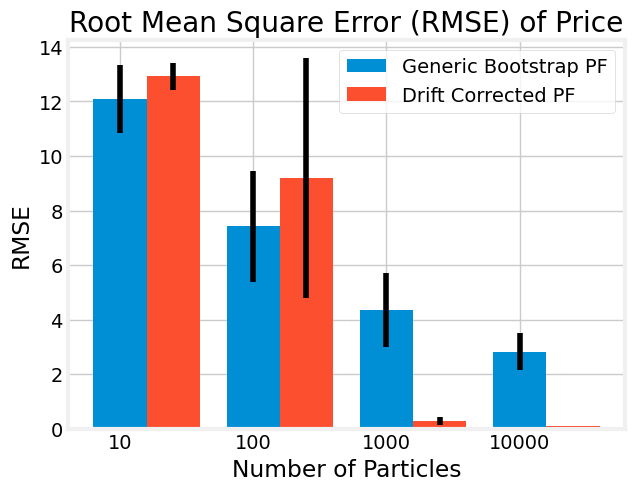
\includegraphics[height=5.5cm]{../plots/4__1__1__bootstrap_comparison_rmse_price.png}}
	\qquad
	\subfloat[RMSE of price($x_1$) state \label{fig:4__1__1__RBPF_comparison_rmse_price}]{
	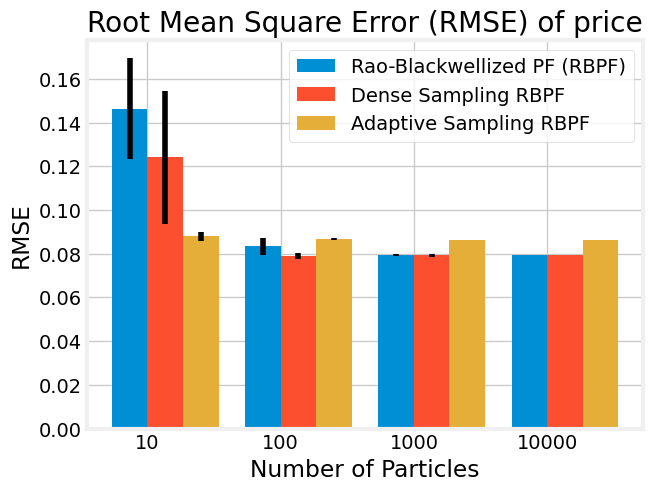
\includegraphics[height=5.5cm]{../plots/4__1__1__RBPF_comparison_rmse_price.png}}
	\\
	\subfloat[RMSE of returns($x_2$)  state \label{fig:4__1__1__bootstrap_comparison_rmse_returns}]{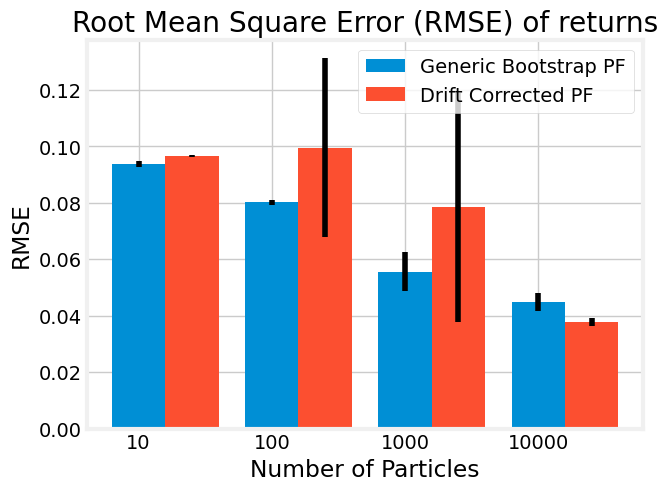
\includegraphics[height=5.5cm]{../plots/4__1__1__bootstrap_comparison_rmse_returns.png}}
	\qquad
	\subfloat[RMSE of returns($x_2$)  state \label{fig:4__1__1__RBPF_comparison_rmse_returns}]{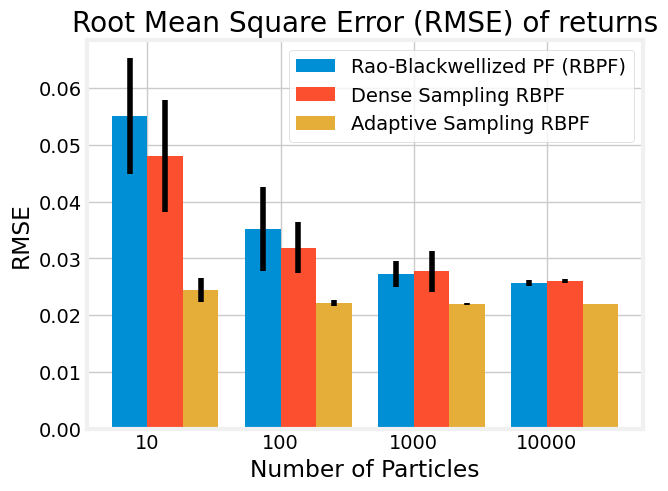
\includegraphics[height=5.5cm]{../plots/4__1__1__RBPF_comparison_rmse_returns.png}}
	\\
	\subfloat[BPE of returns($x_2$)  state \label{fig:4__1__1__bootstrap_comparison_bpe_returns}]{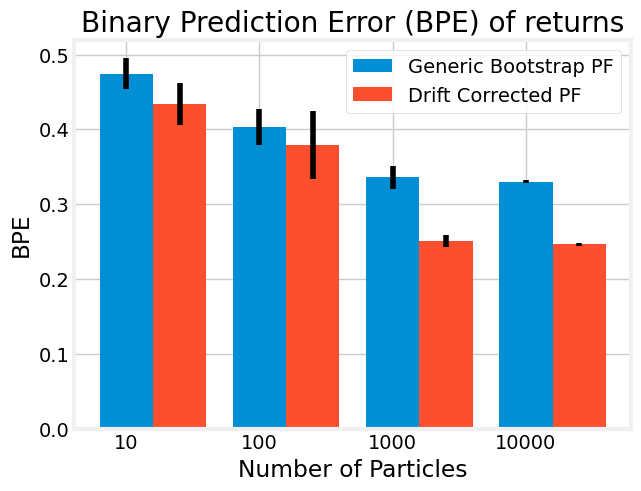
\includegraphics[height=5.5cm]{../plots/4__1__1__bootstrap_comparison_bpe_returns.png}}
	\qquad
	\subfloat[BPE of returns($x_2$)  state \label{fig:4__1__1__RBPF_comparison_bpe_returns}]{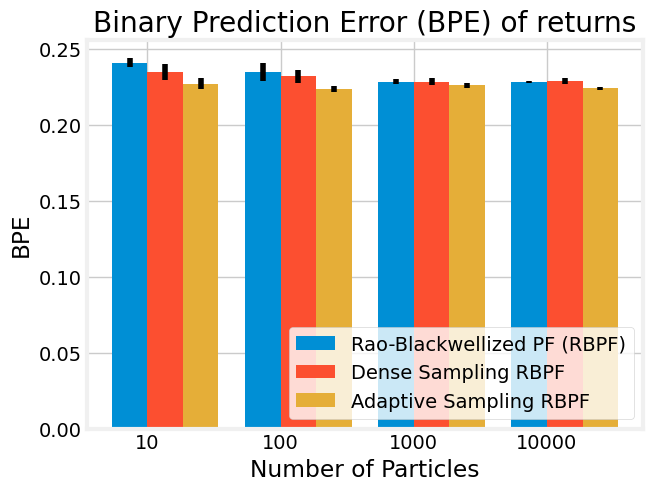
\includegraphics[height=5.5cm]{../plots/4__1__1__RBPF_comparison_bpe_returns.png}}
	\caption{Comparison of inference performance between the 5 inference algorithms as $N$ varies}
	\label{fig:4__1__1__all_comparison}
\end{figure}

\end{document}